\chapter{Existing Solutions for Evaluating Anti-Tracking Tools}
\label{chapter-3}

Establishing a~stable and reproducible testing environment is essential to ensure fair and meaningful comparisons between anti-tracking tools. Such an~environment should include an~automated system that minimizes human interaction and allows for fair and repeatable evaluations of the~anti-tracking capabilities of different browsers and extensions. Since trackers are loaded on web pages accessed through the~browser, the~environment must replicate user activity, such as visiting the~tracking sites with an~automated browser. This chapter presents an~overview of existing tools used to compare the~anti-tracking capabilities of privacy-enhancing tools.

\section{Evaluation Environment}
\label{EnvironmentSection}
The purpose of a~dedicated environment is to make the~results easily replicable. There are two ways to set up such an~environment: following a~detailed set of setup instructions or deploying a~pre-configured environment that is ready to use. Pre-built environments typically come in two forms: through \textit{virtualization} or \textit{containers}.

\subsection{Virtualization}
One of the~ways to create a~replicable environment is by using virtualization~\cite{virtualization}. An~example of virtualization software is \textit{VMware Workstation Pro}\footnote{\url{https://www.vmware.com/products/desktop-hypervisor/workstation-and-fusion/}}. Virtualization allows multiple virtual machines to run concurrently on a~single physical machine. Virtual machines are emulated physical computers that do not need their own hardware to run but instead rely on the~hardware of the~host machines. Host hardware can be shared among multiple virtual machines. 

Virtual machines are controlled by a~\textit{hypervisor} -- software designed to provide a~level of abstraction from the~host system. It also manages the~resources allocated to each virtual machine and prevents virtual machines from affecting each other by isolating them. Figure~\ref{container-and-virtualization-figure} (left) visualizes the~virtualization process. Each virtual machine can run its own operating system, such as \emph{Linux} or \emph{Windows}. Besides that, each virtual machine can be configured for specific purposes, such as running a~web server or, for this thesis, a~comparison of anti-tracking tools. While virtualization is viable, using a~whole virtual operating system may be unnecessarily complex for certain purposes.

\subsection{Containers}
Another method of creating environments is through the~use of containers~\cite{containers}. An~example of container software is \textit{Docker}\footnote{\url{https://www.docker.com/}}. Containers are software that can be executed to run an~application (or multiple applications) they contain. The~code and configuration of each application are included in the~container, together with libraries the~application uses and other required dependencies. Containers rely on operating system-level virtualization, isolating processes from each other and controlling what resources each process can access. Figure~\ref{container-and-virtualization-figure} (right) shows the~container technology. A~practical difference from the~previously mentioned virtualization approach is that containers do not need their own operating system. Instead, they rely on the~host computer's operating system, which makes them less isolated than virtual machines but offers better performance. Relying on the~host operating system makes them more lightweight in terms of both actual size and the~overhead, which is lesser than with virtualization.

\begin{figure}[!ht]
    \centering
    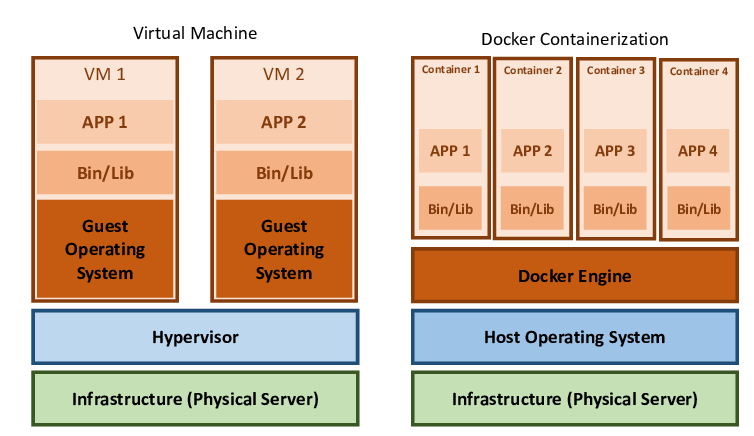
\includegraphics[scale=1.3]{obrazky-figures/Docker-Container-vs-Virtual-Machine.png}
    \caption[Illustration of virtualization and containers]{Illustration\footnotemark{} of virtualization (left) and containers (right).}
    \label{container-and-virtualization-figure}
\end{figure}

\footnotetext{``Docker Container vs. Virtual Machine'' by \emph{Mehr, I. E. et al.} is licensed under \href{https://creativecommons.org/licenses/by/4.0/}{CC BY 4.0}. Retrieved from \url{https://www.researchgate.net/figure/Docker-Container-vs-Virtual-Machine\_fig2\_369061128/} (accessed on \DTMdisplaydate{2025}{04}{16}{-1}).}

\section{Existing Evaluation Methods}
\label{existing-tools-methods}
This section presents several tools and methods that are used to evaluate the~effectiveness of anti-tracking technologies. These tools and methods commonly rely on browser automation to simulate real user activity, such as visiting websites or interacting with elements on a~page. Visiting websites is necessary to trigger tracking scripts and collect data on whether trackers are blocked or whether a~unique and consistent fingerprint can still be generated. A~widely used tool for browser automation in this context is \textit{Selenium}\footnote{\url{https://www.selenium.dev/}}.

\subsection{Straightforward Approach}
The first presented method for benchmarking anti-tracking browser extensions was proposed and implemented by Traverso et al.~\cite{benchmark-method} in 2017. Their method compares anti-tracking performance based on the~number of known trackers contacted during browsing. Their setup uses Selenium to simulate the~Firefox browser. A~list of URLs is used to specify which pages to visit. Each page is visited ten times, with the~browser cache cleared after every visit to ensure consistency. Different privacy-focused extensions are installed and tested one at a~time, each forming a~unique configuration for the~crawl. All HTTP communication between the~browser and the~websites is logged for analysis. The~collected data includes the~number of bytes downloaded, page load times, third-party requests, and contacts with known trackers. These statistics are then used to compare how effectively each extension blocks tracking.
The process moves to the~following URL only after the~current page fully loads, as indicated by the~JavaScript \texttt{onLoad} event. If a~page fails to load correctly, it is skipped and not included in the~results.


\subsection{Open-WPM}
\textit{Open-WPM}~\cite{openwpm}, released in 2016~and still actively maintained as of 2024, is an~open-source tool designed for large-scale web privacy measurements, with its code available at GitHub\footnote{\url{https://github.com/openwpm/OpenWPM}}. The~tool is built to simulate the~user's activity and record data from the~simulated interactions. This data may include cookies, response metadata, and script activity, indicating that the~tool can observe stateful and stateless tracking methods. In addition, OpenWPM can store the~state of the~browser over multiple measurements, allowing it to observe tracking techniques such as cookie respawning, which may be used by evercookies which were described in Subsection \ref{supercookies}. OpenWPM consists of three modules: multiple \textit{browser managers}, \textit{task manager}, and \textit{data aggregator}. Figure~\ref{openwpm-figure} shows the~system's design.

\begin{figure}[!ht]
    \centering
    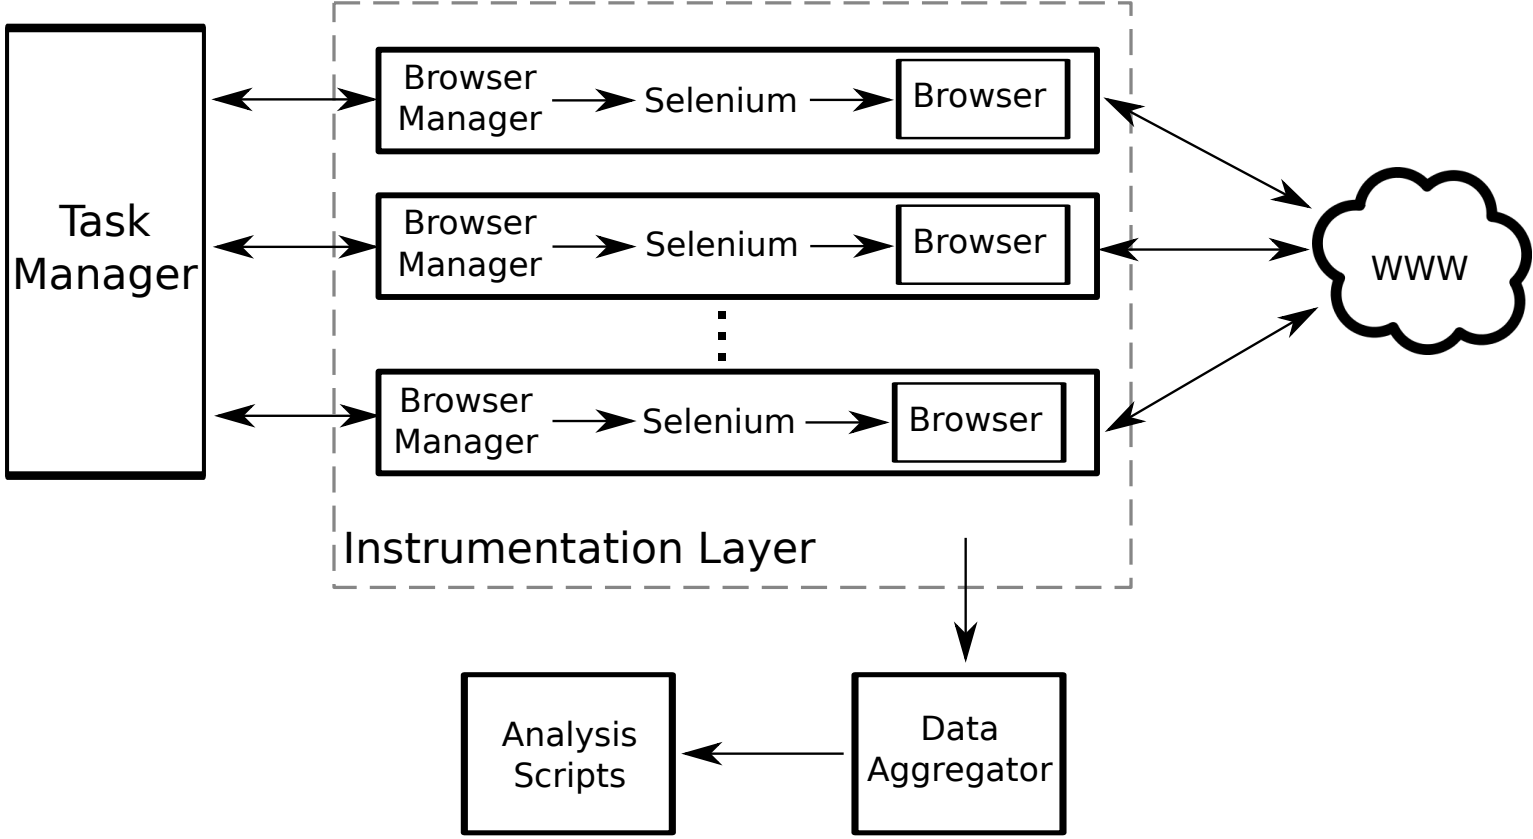
\includegraphics[scale=0.28]{obrazky-figures/openwpm.png}
    \caption[High-level design of OpenWPM]{High-level design of OpenWPM, retrieved from~\cite{openwpm}.}
    \label{openwpm-figure}
\end{figure}

Browser managers run separate instances of full-fledged \textit{Firefox} web browsers via Selenium. Managers are run in parallel to improve performance. When a~new browser manager is created, a~specified configuration is applied. This allows each session to use a~different configuration, such as a~different combination of browser extensions, which may themselves be further configured. In addition, each manager can be configured to perform different tasks. These tasks may consist of, for example, visiting different websites. These managers can also be launched in headless mode, using a~virtual frame buffer for the~graphical interface without displaying it to the~user.

Task manager controls multiple instances of browser managers. Commands for each browser are stored in an~execution thread unique to each browser. If the~browser manager encounters an~error, such as a~timeout or crash, the~current state of the~browser is archived. The~archived state allows the~browser to be restarted later in the~same state (e.g., with cookies stored from visited sites).

Data aggregator stores data received from browser managers. This includes compressed web content, such as all types of cookies (e.g., regular cookies or Flash cookies on legacy systems), HTTP (and HTTPS) request and response headers, and finally, access to various JavaScript prototypes such as storage, canvas, or navigator. The~data is stored in a~structured way, allowing it to be traced back to a~specific browser and page from which it originated. Upon completion, this data can be analyzed to determine, for example, which extension blocked the~most tracking attempts.

\subsection{PETInspector \& FPInspector}
\label{petins-section}
\textit{PETInspector} and \textit{FPInspector}~\cite{petinspector} are used together to form a~benchmarking system, where FPInspector evaluates the~results provided by PETInspector. \textit{PET} stands for \textit{Privacy Enhancing Technology}, and \textit{FP} stands for \textit{Fingerprint}. It was developed in 2019~but has not been updated since. PETInspector is available on GitHub\footnote{\url{https://github.com/tadatitam/pet-inspector}}. The~system can be used to compare different privacy-enhancing extensions and browsers. PETInspector serves as a~tool to experimentally calculate the~anti-fingerprinting capabilities of a~given privacy-enhancing tool, which then forms a~mask of how the~tool behaves. This mask is then used with actual observed fingerprints to simulate how a~browser would behave if everyone were using the~given privacy-enhancing tool. The~resulting traceability is then measured, which is the~purpose of the~FPInspector. This experimental and observational approach forms the~hybrid benchmarking system. The~output of the~system is the~effectiveness of a~given tool. 

The system consists of four parts. These parts are the~\textit{client simulator}, \textit{fingerprinting server} and \textit{analysis engine}, which form the~PETInspector, and the~FPInspector, which is the~fourth part. This is illustrated in the~Figure~\ref{petinspector-figure}.

\begin{figure}[!h]
    \centering
    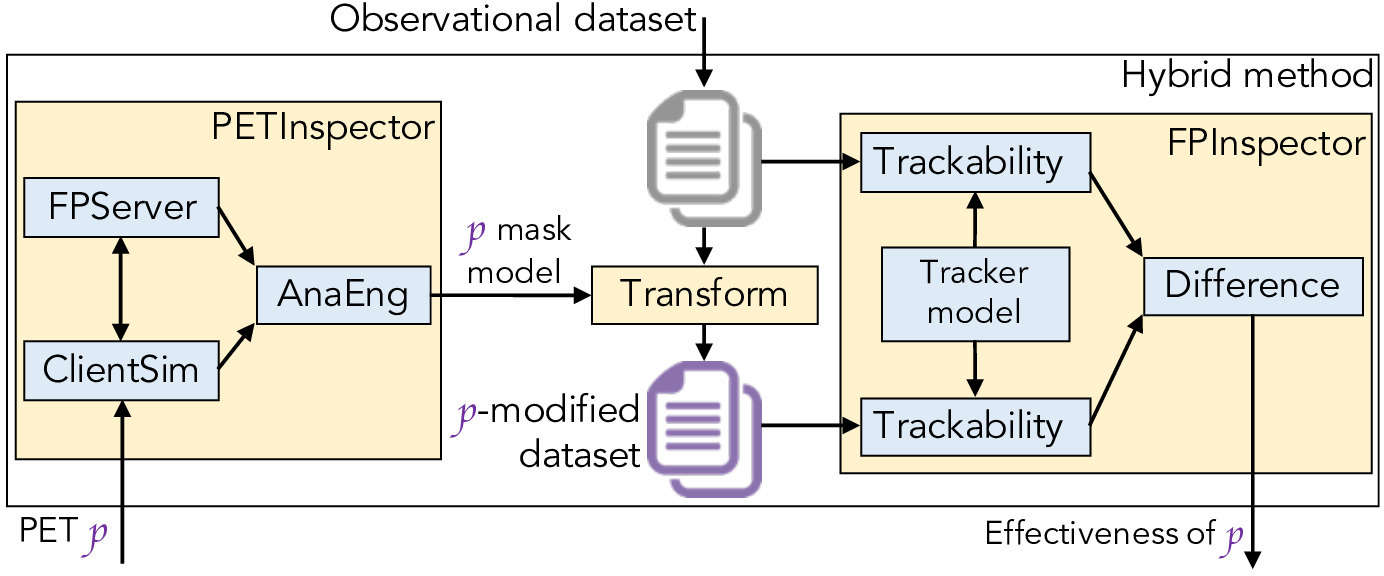
\includegraphics[scale=0.28]{obrazky-figures/petinspector.jpg}
    \caption[Benchmarking system design showcasing how \textit{PETInspector} and \textit{FPInspector} interact]{Benchmarking system design showcasing how \textit{PETInspector} and \textit{FPInspector} interact, retrieved from~\cite{petinspector}.}
    \label{petinspector-figure}
\end{figure}


Client simulator simulates users via Selenium. The~simulator allows the~configuration of different fonts, time zones, and other properties. Each simulated user has various privacy-enhancing tools installed. Additionally, a~client with no privacy-enhancing tools is used to isolate each tool's changes. These simulated users visit the~fingerprinting server, triggering various fingerprinting scripts. The~visits consist of accessing different pages, idling on the~pages, reloading them, and browsing across sessions separated by 45~minutes of downtime.

The fingerprinting server uses various fingerprinting techniques to compute the~fingerprints of visiting clients. The~analysis engine uses information from both the~client simulator and the~fingerprinting server to measure how a~particular client configuration affects a~fingerprint by observing whether the~data the~browser passed to the~fingerprinting server was changed by generalization or randomization. Suppose the~result of the~fingerprinted property is altered by the~privacy-enhancing tool, either by generalization or randomization. In that case, the~property is modeled as masked in the~generated mask and unmasked if not changed. This approach overestimates the~effectiveness because it treats any change to the~property values as unrecoverable, rendering the~property useless for tracking.

FPInspector receives two fingerprint datasets as input. The~first dataset consists of actual measured fingerprints with no privacy-enhancing tool installed. The~second dataset consists of simulated fingerprints, which show what the~first dataset would look like if everyone used a~particular privacy-enhancing tool. The~masks created by PETInspector are used to obtain the~second data set. These datasets are then compared for uniqueness to calculate effectiveness.


\subsection{Browser Extension Testing Environment by Jana Petráňová}
\label{petranova-testing-environment}
This Browser Extension Testing Environment~\cite{petranova-mit} has built-in methods for testing privacy-oriented browser extensions. It does not directly compute the~effectiveness of a~given privacy-oriented tool but returns information about how it affects tracking. It has no official name. The~environment was proposed as part of the~master's thesis by Jana Petráňová~\cite{petranova-mit}. While the~environment is mainly designed to test the~\textit{JShelter} extension, it also supports testing other privacy-oriented extensions. The~extensions can be tested in two supported browsers: Google Chrome and Firefox. It uses the~designs and implementations proposed by \textit{Open-WPM} and \textit{PETInspector} described above. The~environment consists of two main parts: \textit{integration testing} and \textit{system testing}. Its high-level design, together with the~technologies used, is shown in Figure~\ref{petranova-environment}.

Integration testing is based on the~PETInspector tool, described in Subsection \ref{petins-section}. It uses Selenium to simulate a~browser client with privacy-oriented extensions installed. This client visits a~locally hosted website that uses several tracking techniques to generate a~fingerprint. The~server can be customized, though a~default setup is provided. The~server collects various attributes from the~browser, which are stored for later analysis to understand how a~given extension affects the~results returned by various browser methods.

System testing measures how different extensions impact visited web pages. The {\linebreak}Selenium-controlled browser visits a~list of predefined pages, both with and without the~extensions installed. For each visit, the~console output is logged, and a~screenshot is taken before and after applying the~extension. These outputs are then compared to measure how much the~extension changed the~visual layout and behavior of the~page.

\begin{figure}[ht!]
    \centering
    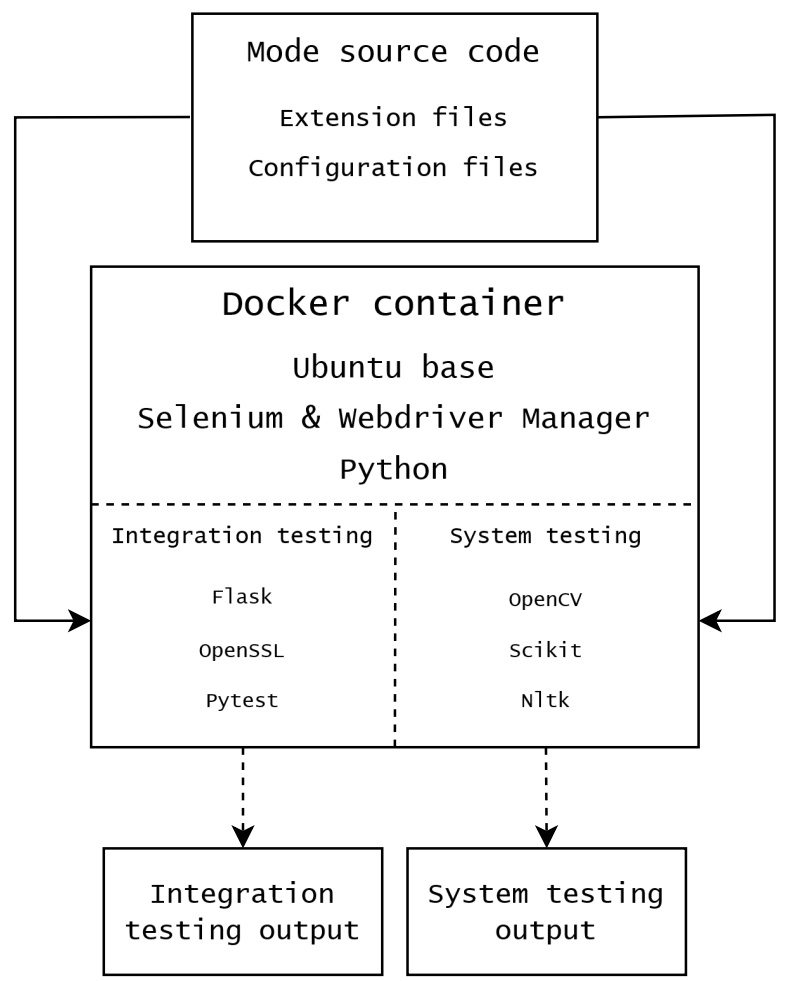
\includegraphics[scale=0.35]{obrazky-figures/petranova.png}
    \caption[Architecture of the~testing environment for anti-tracking tools by\linebreak Jana Petráňová]{Architecture of the~testing environment for anti-tracking tools, retrieved from~\cite{petranova-mit}.}
    \label{petranova-environment}
\end{figure}